\documentclass[11pt, notitlepage]{report}

\usepackage{sectsty}
\usepackage{fancyhdr}
\usepackage{enumitem}
\usepackage{mathtools}
\usepackage{comment}
\usepackage{colortbl}
\usepackage{hyperref}
\usepackage[most]{tcolorbox}
\usepackage{float}
\usepackage{xcolor}
\usepackage{xurl}
\usepackage{amssymb}
\usepackage[a4paper,total={6in,8in}]{geometry}
\usepackage{tikz}
\usepackage{environ}

\renewcommand{\baselinestretch}{1.5} 

\newcommand*\circled[1]{\tikz[baseline=(char.base)]{
            \node[shape=circle,draw,inner sep=2pt] (char) {#1};}}

\newcommand{\RNum}[1]{\uppercase\expandafter{\romannumeral #1\relax}}

\pagestyle{fancy}
\fancyhf{}
\fancyhead[L]{\textbf{\color{doc}{\thesection}}}
\renewcommand{\headrulewidth}{0pt}

\fancypagestyle{plain}{%
  \fancyhf{}% clear all header and footer fields
  \fancyfoot[C]{\bfseries\color{myblue}\thepage}
  \renewcommand{\headrulewidth}{0pt}%
  \renewcommand{\footrulewidth}{0pt}%
}


\newtcolorbox{myproof}[1][]{
    width=\linewidth,
    sharp corners,   
    center,
    colback=gray!35,
    title=\textit{\textbf{Proof:}},
    coltitle=black,colframe=gray!35,
    attach title to upper={\\},
    #1,fontupper=\normalsize,breakable
}


\definecolor{myblue}{rgb}{0.44, 0.65, 0.82}
\definecolor{doc}{HTML}{191971}
\sectionfont{\color{doc}}
\subsectionfont{\color{doc}}
\subsubsectionfont{\color{doc}}
\chapterfont{\color{doc}}

\newtagform{myblue}[\textcolor{myblue}]{\color{myblue}(}{)}
\usetagform{myblue}

% Define colors for theorem and proof boxes
\definecolor{theorembg}{RGB}{240,248,255} % Light blue for theorem background
\definecolor{theoremframe}{RGB}{0,100,180} % Darker blue for theorem frame
\definecolor{proofbg}{RGB}{255,250,205}   % Light yellow for proof background
\definecolor{proofframe}{RGB}{180,100,0}  % Darker yellow for proof frame

% Theorem environment definition
\newtcolorbox[auto counter, number within=section]{theorem}{
    width=\textwidth,
    sharp corners,
    center,
    colback=myblue!20,
    colframe=myblue,
    breakable, % Allows box to break across pages if needed
    enhanced,  % Improves appearance and allows for better customization
    title={Theorem \thetcbcounter:},
    fonttitle=\bfseries,coltitle=black,attach title to upper={\\},fontupper=\normalsize,breakable,
}

% Theorem environment definition
\newtcolorbox[auto counter, number within=section]{prop}{
    width=\textwidth,
    sharp corners,
    center,
    colback=myblue!20,
    colframe=myblue,
    breakable, % Allows box to break across pages if needed
    enhanced,  % Improves appearance and allows for better customization
    title={Proposition \thetcbcounter:},
    fonttitle=\bfseries,coltitle=black,attach title to upper={\\},fontupper=\normalsize,breakable,
}

% Proof environment definition (nested within theorem)
\newtcolorbox{proof}{
    width=\linewidth,
    sharp corners,   
    center,
    colback=gray!20,
    title=\textit{Proof:},
    coltitle=black,colframe=gray!35,
    attach title to upper={\\},fontupper=\normalsize,enforce breakable, break at=18cm
}



% Definition environment definition
\newtcolorbox[auto counter, number within=section]{definition}{
    width=\textwidth,
    sharp corners,
    center,
    colback=white,
    colframe=black,
    breakable, % Allows box to break across pages if needed
    enhanced,  % Improves appearance and allows for better customization
    title={Definition \thetcbcounter:},
    fonttitle=\bfseries,coltitle=black,attach title to upper={\\},fontupper=\normalsize,
}

\geometry{
 a4paper,
 total={170mm,257mm},
 left=20mm,
 top=20mm,
 }

\usepackage{titlesec}

\titleformat{\chapter}[display]
  {\color{doc}\normalfont\bfseries}{}{0pt}{\huge}

  \usepackage[dvipsnames]{xcolor}

\usepackage{tocloft}

\renewcommand\cfttoctitlefont{\Large\bfseries\color{doc}}
\renewcommand\cftaftertoctitle{\hfill\mbox{}}
\cftsetindents{section}{0em}{2em}
\cftsetindents{subsection}{0em}{2em}
\setlength{\cftaftertoctitleskip}{-1em}



\begin{document}

\title{Math Notes}
\author{Matthew Satter}
\date{\today}
\maketitle
\vspace{-2cm}
{\let\clearpage\relax \tableofcontents}

\thispagestyle{empty}

\chapter{Complex Analysis Review}

\chapter{Manifolds and Riemann Surfaces}

\pagestyle{fancy}
\fancyfoot{}
\fancyhead[L]{\normalsize\textbf{\textcolor{doc}{\rightmark}}}
\fancyfoot[C]{\bfseries\color{myblue}\thepage}

\setcounter{page}{1}

\section{The Big Idea}

A \textbf{\textcolor{myblue}{Riemann surface}} is a surface that locally looks like open subsets of $\mathbb{C}$. By ``looks like'' an open subset of $\mathbb{C}$, we mean that a Riemann surface is a \textbf{\textcolor{myblue}{topological surface}}, or \textit{a two-dimensional real manifold} (meaning neighborhoods on the surface map to open subsets of the Euclidean plane), but Riemann surfaces also have a so called \textbf{\textcolor{myblue}{``complex structure''}}, meaning that we can perform complex analysis on the surface. This structure distinguishes Riemann Surfaces from other two-dimensional real manifolds. 

For instance, we want to find a way to define ``holomorphic functions'' on such Riemann surfaces. But holomorphic functions are only defined on complex-valued functions with \textit{complex inputs}, so how could we define the idea of holomorphicity on surfaces instead?

Well, suppose we have a function defined from a open ``disk-like'' subset $D$ of a surface $S$ that takes complex values, i.e. $f:D\rightarrow\mathbb{C}$. To determine if $f$ is ``holomorphic'', we first see if we can bijectively identify with each point on $D$ a corresponding point in $\mathbb{C}$. Traditionally, we seek bijections $\phi:D\to \mathbb{D}$, where $\mathbb{D}$ is the open unit disk in $\mathbb{C}$. We could then define that $f$ is \textbf{\textcolor{myblue}{holomorphic}} if the composition of maps $f\circ\phi^{-1}:\mathbb{D}\to\mathbb{C}$ is itself holomorphic as a complex valued function with complex inputs. 

\begin{figure}[H]\begin{center}
    \fbox{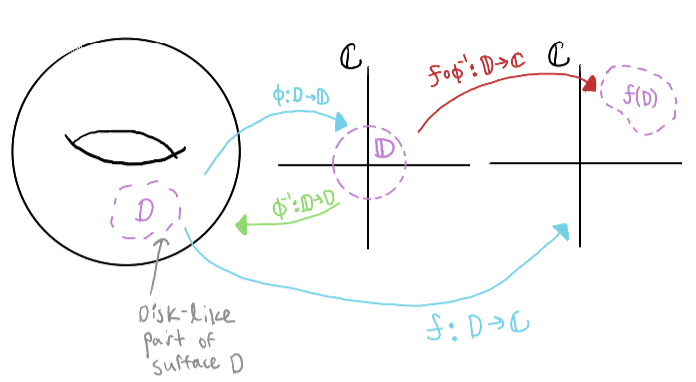
\includegraphics[width=0.5\textwidth]{Images/bigidea.png}}
\end{center}\caption{To ``perform'' complex analysis on surfaces, we map parts of the surface to the unit disk $\mathbb{D}$ via a biholomorphism $\phi$. The resulting complex analysis is performed on the function $f\circ \phi^{-1}$.}\end{figure} To more carefully describe this notion, we proceed with some review in the next section before formally defining a Riemann Surface.

\section{Homeomorphisms}
\begin{definition}A \textbf{\textcolor{myblue}{topological space }} is a pair $(X,\tau)$ consisting of a set $X$ and a corresponding \textbf{\textcolor{myblue}{topology}} $\tau$ on $X$, (here $\tau$ is a collection of subsets of $X$, i.e. $\tau\in 2^X$), where the topology $\tau$ obeys the following properties: \begin{itemize}\setlength{\itemsep}{.1ex}\item The empty set $\varnothing$ and $X$ are in $\tau$. \item The union of \textit{any} collection of sets in $\tau$ is also in $\tau$. \item The intersection of any \textit{finite} collection of sets in $\tau$ is also contained in $\tau$.  \end{itemize}  \end{definition}


\begin{definition} A \textbf{\textcolor{myblue}{homeomorphism}} is a bijective function with a continuous inverse. If there is a homeomorphism from one topological space $X$ to another topological space $Y$ we say are topological spaces are \textit{homeomorphic}.
\end{definition}

\noindent\textbf{Example: }The function $\tan: (-\pi/2,\pi/2)\to\mathbb{R}$ is a homeomorphism.


\noindent \textbf{Note: }Rescaled tangent and arctangent functions (or other continuous monotone functions) can be used to make homeomorphisms from any open interval contained in $\mathbb{R}$ to $\mathbb{R}$ itself. One can show that any two open intervals in $\mathbb{R}$ are homeomorphic.

\noindent There are many homeomorphisms, and perhaps it is more interesting to consider some nonexamples of homeomorphisms.

\noindent \textbf{Nonexample: }
    The function $f:[0,2\pi)\to S^1$ (the unit circle) given by $f(\theta)=(\cos(\theta),\sin(\theta))$ is continuous and invertible, but its inverse is not continuous as $f^{-1}((1,0))=0$, but for any neighborhood of $(1,0)$ on the unit circle, there are points mapped by $f^{-1}$ near both $0$ and $2\pi$. This says that the unit circle is not homeomorphic to a line segment (you cannot continuously deform the unit circle into a line segment without ``cutting'').

\noindent If topological spaces are homeomorphic, it turns out that they share the same topological properties (connectedness, compatnesss, etc.), but we will not prove this here. We want to move to studying similar concepts but on the complex plane and with a slightly stronger property than homeomorphicity.

\section{Complex Analysis Review}

To motivate this review, fix an open subset $\Omega\subseteq \mathbb{C}$ and a point $z_0\in \Omega$. Suppose a function $f: \Omega\rightarrow \mathbb{C}$ is complex differentiable at $z_0$, and $\gamma:(a,b)\to\mathbb{C}$ is a differentiable curve with $\gamma(t_0)=z_0$ for some $t_0\in(a,b)$. The chain rule tells us \begin{equation}
    (f\circ\gamma)'(t_0)=f'(\gamma(t_0))\gamma'(t_0)
\end{equation}
If $f'(z_0)\neq 0$ and $\gamma'(t_0)\neq 0$, then we can write \begin{equation}
    \arg(f\circ\gamma)'(t_0)=\arg(f'(z_0))+\arg(\gamma'(t_0)),\label{argsplit}
\end{equation} which tells us that for any curve $\gamma$ passing through $z_0$, the tangent vector $\gamma'(t_0)$ is rotated counterclockwise by the angle $\arg(f'(z_0))$. Note that any such curve passing through $z_0$ (with nonvanishing derivative) is rotated by the same angle (i.e. the angle depends only on $z_0$). This means that if $\gamma_1$ and $\gamma_2$ are any two curves passing through $z_0$ (assume $\gamma_1(t_1)=\gamma_2(t_2)=z_0$) with $\gamma_1'(t_1)\neq0 $ and $\gamma_2'(t_2)\neq 0$, if a function $f$ is such that $f'(z_0)\neq 0$, then we can write \begin{equation}\arg(f\circ\gamma_1)'(t_1)-\arg(f\circ\gamma_2)'(t_2)=\arg(\gamma_1'(t_1))-\arg(\gamma_2'(t_2))\end{equation} so such a map with nonzero derivative preserves angles between curves. We say such maps are conformal, and this concept motivates the definition below.

\begin{definition}Let $\Omega$ be a region (open nonempty connected subset) of $\mathbb{C}$ and let $$g:\Omega\to\mathbb{C}$$ be a continuously differentiable function in the real sense. That is to say that if we write the function $g(x+iy)=u(x,y)+iv(x,y)$ where $u$ and $v$ are real-valued functions with real inputs, then $u$ and $v$ have continuous partial derivatives and the derivative matrix  $\begin{bmatrix}\dfrac{\partial u}{\partial x}&\dfrac{\partial u}{\partial y}\\\dfrac{\partial v}{\partial x}&\dfrac{\partial v}{\partial y}\end{bmatrix}$ consequently exists as a linear transformation on the plane. 

Let $z_0$ be some point in $\Omega$. We say that the function $g$ is \textbf{\textcolor{myblue}{conformal at $z_0$}} if there exist numbers $$r\in(0,\infty)\hspace{1cm}\text{and}\hspace{1cm}\theta\in[0,2\pi)$$ such that for any interval $I$ and differentiable curve $\gamma:I\to\Omega$ with $\gamma(t_0)=z_0$, then \begin{equation}
    |(g\circ\gamma)'(t_0)|=r\cdot|\gamma'(t_0)|,\hspace{1cm}\text{and}\hspace{1cm}\arg((g\circ\gamma)'(t_0))=\theta+\arg(\gamma'(t_0)).\label{conformal}
\end{equation}
We say $g$ is \textbf{\textcolor{myblue}{conformal}} if it is conformal at each point in $\Omega$. 
\end{definition}

This definition says that for any curve $\gamma$ passing through a point $z_0$, once fed into a conformal map $g$, the tangent vector to $\gamma$ at $z_0$ is stretched by some factor $r$ and rotated by some angle $\theta$, where $r$ and $\theta$ are \textit{independent} of the specific choice of curve $\gamma$. Rather, $r$ and $\theta$ only depend on $g$ and $z_0$, as we will see in further detail below.

\begin{theorem}
    Let $\Omega\subseteq \mathbb{C}$ be a region, and $g:\Omega\to\mathbb{C}$ be a continuously differentiable function in the real sense. Let $z_0$ be any point in $\Omega$. Then $g$ is conformal at $z_0$ if and only if it is complex differentiable at $z_0$ and $g'(z_0)\neq 0$. \begin{proof}
        As $g$ is real-differentiable on $\Omega$, if $z_0=x_0+iy_0$, then for any differentiable curve $\gamma=(\gamma_1(t),\gamma_2(t))$ with $\gamma(t_0)=(x_0,y_0)$, the real-derivative of $g$ at $z_0$ is given by the chain rule: \begin{equation}
    (g\circ\gamma)'(t_0)=g'(z_0)\gamma'(t_0),\label{chainrule}
\end{equation}where here the notation $g'(z_0)$ denotes the real-derivative matrix evaluated at the point $(x_0,y_0)$ and $\gamma'(t_0)=(\gamma_1'(t_0),\gamma_2'(t_0))^T$ is the component-wise time-derivative of $\gamma$ evaluated at $t_0$. 

If $g$ is conformal, then definition above tells us that the tangent vector $\gamma'(t_0)$ is scaled by $r\in(0,\infty)$ and rotated by an angle of $\theta\in[0,2\pi)$. Looking at the equation above, it must consequently be that $g'(z_0)$ has the form of a scaled rotation matrix, or more explicitly:\begin{equation}g'(z_0)=r\begin{bmatrix}\cos\theta&-\sin\theta\\\sin\theta&\cos\theta\end{bmatrix}.\end{equation}For $r\in(0,\infty)$ and $\theta\in[0,2\pi)$, we could then rewrite the equation above in the form \begin{equation}g'(z_0)=\begin{bmatrix}a&-b\\b&a\end{bmatrix}\text{ for some $a$,$b\in\mathbb{R}$, not both zero.}\end{equation} But this form lets us see that if $g(x+iy)=u(x,y)+iv(x,y)$, then $\dfrac{\partial u}{\partial x}(x_0,y_0)=\dfrac{\partial v}{\partial y}(x_0,y_0)$ and $\dfrac{\partial u}{\partial y}(x_0,y_0)=-\dfrac{\partial v}{\partial x}(x_0,y_0)$, so the Cauchy-Riemann equations are satisfied. Since $g$ satisfies the Cauchy-Riemann equations at $z_0$ (and $u,v$ have continuous partials), then we know $g$ is \textit{complex differentiable} at $z_0$. Furthermore, since $a$ and $b$ are not simultaneously zero, then $g'(z_0)=a+ib\neq 0$. 

For the reverse implication, if $g'(z_0)$ exists and is nonzero, we can write $g'(z_0)=re^{i\theta}$ for some $r\in(0,\infty)$ and $\theta\in[0,2\pi)$. Then, if we take modulus and arguments of both sides of \eqref{chainrule} we see that the conditions \eqref{conformal} are satisfied, so $g$ is indeed conformal at $z_0$.
    \end{proof}
\end{theorem}


\noindent {\normalsize \textbf{\underline{Note:} } Some functions like $\overline{z}$ are called \textit{anticonfomal}  as they reverse the angles between curves (as  $\arg(\overline{z})=-\arg z$). Note that such maps are notoriously not conformal. For example, $\overline{z}$ is nowhere complex differentiable and thus cannot be conformal by the characterization above.}

\begin{definition} Let $\Omega\subseteq \mathbb{C}$ be a nonempty open set, and let $z_0\in\Omega$. A function $f:\Omega\to\mathbb{C}$ is \textbf{\textcolor{myblue}{holomorphic at $z_0$}} if there exists a radius $r>0$ such that the neighborhood $\mathbb{D}_r(z_0)$ is contained in $\Omega$ and such that $f$ is complex differentiable on $\mathbb{D}_r(z_0).$ We say $f$ is \textbf{\textcolor{myblue}{holomorphic}} if it is holomorphic at all points in $\Omega$. 
\end{definition}

\noindent To begin studying relationships between holomorphic and conformal maps, we will first prove that injective holomorphic maps have nonvanishing derivative (and are thus conformal). This is yet another miraculous fact in complex analysis, as in real analysis there are many functions that are injective and differentiable and yet have vanishing derivative (like $x\mapsto x^3$ for instance).

\begin{theorem}
    For a domain $\Omega$, if a function $f:\Omega\to\mathbb{C}$ is injective and holomorphic, then it has nonvanishing derivative, and is thus conformal. \begin{proof}  We wish to show that $f$ is conformal, so it will suffice to show that $f'(z)\neq 0$ on $\Omega$. We proceed by contradiction, and assume there is a $z_0\in\Omega$ such that $f'(z_0)=0$. Then we define the auxiliary function $g(z)=f(z)-f(z_0)$. Note that $g(z_0)=f(z_0)-f(z_0)=0$ and also that $g'(z_0)=f'(z_0)=0$. Since this auxiliary function $g$ is holomorphic (and thus analytic), we can Taylor expand \begin{equation}g(z)=(z-z_0)^2\sum_{j=0}^\infty\dfrac{g^{(2+j)}(z_0)}{(2+j)!}(z-z_0)^j\end{equation}So it must be that $g$ has a repeated zero (i.e. of multiplicity $\geq 2$) at $z_0$. Non-constant holomorphic/analytic functions have isolated zeros.  
    \end{proof}
\end{theorem}



\begin{definition} A \textbf{\textcolor{myblue}{biholomorphism}} is a bijective holomorphic function with a holomorphic inverse.   
\end{definition}


\noindent The Proposition above immediately tells us that \textit{\textbf{all biholomorphisms are conformal}}.

\section{Complex Charts}
\begin{definition}[] A \textbf{\textcolor{myblue}{complex coordinate chart}} (or patch) is a pair $(U,\phi)$ consisting of some open subset $U$ of a topological space $X$ and a homeomorphism $\phi:U\to V$ where $V$ is an open subset of the complex plane.\end{definition}

\noindent \textbf{Example: }
    The relabeling of any open subset $U$ of $\mathbb{R}^2$ (i.e. $U\subseteq X=\mathbb{R}^2$) as as subset of $\mathbb{C}$ through the chart $\phi_U(x,y)=x+iy\in\mathbb{C}$.

\noindent \textbf{Example: }
    The mapping of any open subset $U$ of $\mathbb{R}^2$ (i.e. $U\subseteq X=\mathbb{R}^2$) to a subset of $\mathbb{D}=\{z\in\mathbb{C}:|z|<1\}$ through the chart $\phi_U(x,y)=\dfrac{x}{1+\sqrt{x^2+y^2}}+i\dfrac{y}{1+\sqrt{x^2+y^2}}\in\mathbb{C}$. \newline {\normalsize \textbf{\underline{Note:} } In polar coordinates, this chart is $\phi_U(r,\theta)=\dfrac{r}{r+1}e^{i\theta}$, so $\phi(\mathbb{C})=\mathbb{D}$. And, $\phi_U^{-1}(u+iv)=\left(\dfrac{u}{1-\sqrt{u^2+v^2}},\dfrac{v}{1-\sqrt{u^2+v^2}}\right)$.\newline \textbf{\underline{Note:} } If considered as a complex-valued function with complex inputs, $\phi_U(z)=\dfrac{z}{1+|z|}$ is a homeomorphism from $\mathbb{C}$ to $\mathbb{D}$. However, it is \textbf{nowhere} complex differentiable, as $|z|$ is nowhere complex differentiable. We will learn later that it is impossible to create a biholomorphism from $\mathbb{C}$ to $\mathbb{D}$.}



\begin{definition} For a topological space $(X,\tau)$, an  \textbf{\textcolor{myblue}{atlas}} is a collection of coordinate charts that covers $X$. More specifically, for an index set $I$, an atlas $A=\left\{\left(U_\alpha,\phi_\alpha\right):\alpha\in I\right\}$ where each $(U_\alpha,\phi_\alpha)$ is a coordinate chart and $\bigcup_{\alpha\in I}U_\alpha= X$.\end{definition}

\begin{definition} A \textbf{\textcolor{myblue}{manifold}} is a pair $(\mathcal{M},A)$ consisting of a topological space $\mathcal{M}$ and an atlas $A$ for $\mathcal{M}$. \end{definition}



There are several classifications of manifolds, and entire courses on smooth manifolds, (real) analytic manifolds, and so forth. Our primary discussion will involve complex manifolds instead.


\begin{definition}A \textbf{\textcolor{myblue}{complex manifold}} is a manifold $(\mathcal{M},A)$ consisting of a topological space $\mathcal{M}$ and an atlas $A$ of biholomorphic charts that map to the unit disk $\mathbb{D}:=\{z\in\mathbb{C}: |z|<1\}$ in the complex plane.\end{definition}

An initial question to ask is why this definition involves charts to the unit disk and not to the entirety of $\mathbb{C}$ itself. This goes back to the ``big idea'' described at the very the beginning. We want to start with a ``disk-like'' patch of a surface $D\subset\mathbb{R}^3$, and first map $D$ to $\mathbb{D}$ via a biholomorphism $\phi$. Then, we wish to define a function $f:D\to\mathbb{C}$ as holomorphic if  $f\circ\phi^{-1}:\mathbb{D}\to\mathbb{C}$ is holomorphic.

If we saught biholomorphic charts $\phi$ from the ``disk-like'' part of the surface $D$ to $\mathbb{C}$ outright, we would encounter problems. For instance, if we want to define $\mathbb{D}$ itself as a complex manifold, seeking biholomorphisms $\phi$ from $\mathbb{D}$ to $\mathbb{C}$ outright raises concerns as $\phi^{-1}:\mathbb{C}\to\mathbb{D}$ would be an entire function and would be such that $\sup_{z\in \mathbb{C}}|\phi^{-1}(z)|\leq 1$. Thus, $\phi^{-1}$ would be a bounded entire function and constant by Liouville's theorem. But then $\phi$ could not possibly be a chart since constant functions are non-invertible.

For this reason, to be able to define $\mathbb{D}$ itself as a complex manifold, it is standard to use it (or perhaps another bounded subset of $\mathbb{C}$) as the codomain for our biholomorphic charts in our definition.

In general we will cover our surfaces with many complex coordinate patches, and might wonder if using different coordinate charts on the same part of the surface could potentially lead to problems. We will say that two coordinate patches are ``compatible'' if they either do not overlap, or if we can map biholomorphically from one to the other (meaning we can effectively go back and forth between the two without consequence). This is laid out in detail in the definition below, and pictured in Figure \ref{fig:1.2}. One can think of the difference between compatible charts as a simple change of coordinates and nothing more.
\begin{figure}[H]\begin{center}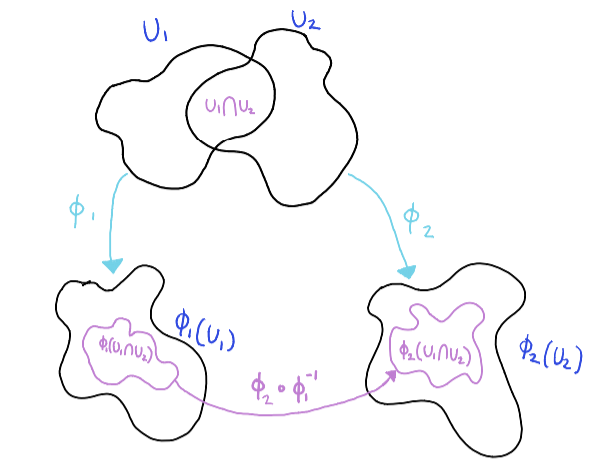
\includegraphics[scale=0.8]{Images/compatibility.png}\end{center}\caption{Charts are compatible if they do not overlap or we can go biholomorphically from one to the other.}\label{fig:1.2}\end{figure}

\begin{definition} Let $(U_1,\phi_1)$ and $(U_2,\phi_2)$ be two complex coordinate charts. We say that the charts $\phi_1$ and $\phi_2$ are \textbf{\textcolor{myblue}{compatible}} if either $U_1\cap U_2=\varnothing$, or $\phi_2\circ\phi_1^{-1}:\phi_1(U_1\cap U_2)\to \phi_2(U_1\cap U_2)$ is holomorphic.
\end{definition}

In the definition above, we need only worry about defining one direction $\phi_2\circ\phi_1^{-1}$, due to the proposition below.
\begin{prop}
    For complex homeomorphisms $\phi_1,\phi_2$, if $\phi_2\circ\phi_1^{-1}$ is holomorphic on $\phi_1(U_1\cap U_2)$, then $\phi_1\circ\phi_2^{-1}$ is holomorphic on $\phi_2(U_1\cap U_2)$. \begin{proof}If $\phi_2\circ\phi_1^{-1}$ is holomorphic, the complex chain rule gives us that $(\phi_2\circ\phi_1^{-1})'(z)=\dfrac{\phi_2'(\phi_1^{-1}(z))}{\phi_1'(\phi_1^{-1}(z))}$.\end{proof}
\end{prop}









\newcommand{\vu}{\vec{u}}
\newcommand{\nhat}{\widehat{n}}
\newcommand{\pd}[2]{\df{\partial {#1}}{\partial {#2}}}
\newcommand{\lp}{\left(}
\newcommand{\rp}{\right)}
\newcommand{\df}[2]{\dfrac{{#1}}{{#2}}}
\newcommand{\beq}{\begin{equation}}
\newcommand{\eeq}{\end{equation}}

\newcommand{\ds}{\displaystyle}

\numberwithin{equation}{chapter}

\def\resetstyle#1{{\normalsize\rm\color[rgb]{0,0,0}\noindent#1}}



\chapter{Riemann Surfaces}

\section{Stereographic Projection}



Consider $\mathbb{R}^3$, and let $\mathbb{C}=\left\{(x_1,x_2,x_3)\in\mathbb{R}^3: x_3=0\right\}$ so that the complex plane is viewed as the $x_1x_2$-plane in $\mathbb{R}^3$. Also, let $S^2=\left\{(x_1,x_2,x_3)\in\mathbb{R}^3: x_1^2+x_2^2+x_3^2=1\right\}$ be the standard unit sphere and let $\vec{N}=\left(0,0,1\right)$ be the ``north pole'' of the unit sphere.

We seek to project points from $S^2\setminus \vec{N}$ to $\mathbb{C}$ by drawing a projective line through $\vec{N}$ and $\vec{x}\in S^2\setminus \vec{N}$ and then finding the point $p(\vec{x})\in\mathbb{C}$ where the projective line intersects the complex plane. To find a formula for such a mapping, we could first consider the inverse mapping. Given $z=z_1+iz_2\in\mathbb{C}$, what $\vec{x}\in S^2\setminus\vec{N}$ gets projected there?

To find this inverse mapping, we first parameterize the line segment $\vec{\ell}$ connecting $\vec{N}$ to $z$ by $\vec{\ell}(t)=\left\{\begin{bsmallmatrix}0\\ \\ 0\\\\1\end{bsmallmatrix}t+{\begin{bsmallmatrix}z_1 \\ \\ z_2 \\ \\ 0 
\end{bsmallmatrix}}\left(1-t\right):t\in[0,1]\right\}.$ To find where this line segment intersects the unit sphere, we look for a $t_0$ in $(0,1)$ such that $\left|\left|\vec{\ell}(t_0)\right|\right|=1$. This gives us that $t_0^2+|z|^2(1-t_0)^2=1$ and after moving things around that $|z|^2(1-t_0)^2=1-t_0^2$. Factoring the left side gives us \begin{equation}
    |z|^2(1-t_0)^2=(1+t_0)(1-t_0).\label{st1}
\end{equation} 

If $t_0=1$, since $\vec{\ell}(1)=\vec{N}$, then the projective line would intersect the north pole with a multiplicity of two, (and thus the projective line would be tangent to $S^2$ at the north pole). In this case, we will say that the projective line intersects $\mathbb{C}$ at $\infty$ in the extended complex plane, but cannot intersect at any $z$ in the complex plane.

Since we assumed the projection point actually lives in $\mathbb{C}$, then we can assume $t_0\neq 1$, and can divide both sides of equation \eqref{st1} by $1-t_0$ to get \begin{equation}\begin{split}|z|^2(1-t_0)&=1+t_0\\|z|^2-1&=t_0(1+|z|^2)\\t_0&=\dfrac{|z|^2-1}{|z|^2+1}.\\\end{split}\end{equation}

We then see that the point on $S^2$ projected to $z$ is given by \begin{equation}\vec{\ell}(t_0)=\left(\dfrac{2z_1}{|z|^2+1},\dfrac{2z_2}{|z|^2+1},\dfrac{|z|^2-1}{|z|^2+1}\right)=\left(\dfrac{z-\overline{z}}{|z|^2+1},\dfrac{-i(z-\overline{z})}{|z|^2+1},\dfrac{|z|^2-1}{|z|^2+1}\right).\end{equation} To get our original projection mapping, we can look for an inverse. If $x_1=\df{2z_1}{|z|^2+1}$, $x_2=\df{2z_2}{|z|^2+1}$ and $x_3=\df{|z|^2-1}{|z|^2+1}$, note that \begin{equation}1-x_3=\dfrac{|z|^2+1-\left(|z|^2-1\right)}{|z|^2+1}=\df{2}{|z|^2+1}=\df{x_1}{z_1}=\df{x_2}{z_2}.\end{equation}

So as long as $x_3\neq 1$ (which once again is true as long as the projective line is not tangent to the north pole), we can say $z_1=\df{x_1}{1-x_3}$ and $z_2=\df{x_2}{1-x_3}$. We summarize this derivation formally with the following definitions:

\begin{definition}[]
    The \textbf{\textcolor{myblue}{stereographic projection}} is a map $p_+:S^2\setminus\vec{N}\to \mathbb{C}$ defined by \begin{equation}p_+((x_1,x_2,x_3))=\df{x_1+ix_2}{1-x_3}.\end{equation}
\end{definition}
The ``+'' subscript on the stereographic projection indicates that the north pole was used as one of the projective line points. Repeating the derivation with the south pole gives an alternate projection $p_-((x_1,x_2,x_3))=\df{x_1+ix_2}{1+x_3}$. 

\begin{definition}The \textbf{\textcolor{myblue}{extended complex plane}} $\widehat{\mathbb{C}}$ is the set $\widehat{\mathbb{C}}=\mathbb{C}\cup\{\infty\}$.
\end{definition}


\section{Riemann Surfaces}

\include{Exercises}

\end{document}
